\chapter{INTRODUCTION}

\section{Introduction}
\hspace{12pt} Earthquakes, as significant natural disasters, present unique challenges due to their unpredictability. This unpredictability of earthquakes poses a formidable challenge in mitigating their impact on communities and infrastructure. Acknowledging the pressing demand for effective solutions, \ac{EEWs} have become indispensable for issuing alerts before the arrival of seismic waves. In the realm of seismic activity, two distinct types of waves play pivotal roles. The first, P-waves, possess greater speed at approximately 6 km/s but are characterized by a relatively weaker impact. In contrast, the second type, S-waves, move at a slower pace at approximately 3 km/s but are notably more destructive. \ac{EEWs} operate on a crucial distinction – they do not predict earthquakes. Instead, their functionality lies in the rapid identification of seismic waves as soon as an earthquake initiates. Once seismic waves are detected, \ac{EEWs} swiftly engages in the process of expediently transmitting alerts. This proactive approach ensures that individuals and communities receive timely notifications, allowing them precious seconds to initiate preparatory measures before the actual tremor reaches their vicinity.\\

Nevertheless, current \ac{EEWs} face significant drawbacks. While these systems typically rely on established telecommunication infrastructure like mobile networks and internet services, their effectiveness can be compromised during an earthquake. The seismic activity may lead to damage or failure of telecommunication networks, rendering the warning system inoperable and highlighting a critical vulnerability in the current approach.\\

The constraints inherent in current \ac{EEWs} underscore the urgent need for alternative solutions that enhance reliability and resilience. In response to this imperative, we propose a communication architecture founded on LoRa technology which is an independent telecommunication method not reliant on traditional telecommunication infrastructure. LoRa, or Long Range Radio, offers a low-power, long-range communication approach capable of transmitting low bit rates over substantial distances. Further details on LoRa are elaborated in subsequent sections.\\

Our suggested architecture serves as a redundant communication method for existing \ac{EEWs}, addressing the vulnerabilities associated with communication networks in current \ac{EEWs}. Notably, this proposed solution can be implemented at a relatively low cost, making it a feasible and practical addition to bolster the robustness of current earthquake warning systems.\\

In this study, we are not considering earthquake detection or verification. Instead, our attention is solely on how warning messages are transmitted upon the detection and verification of earthquakes. Specifically, we are concerned with latency. Given that the P-wave is weaker, we assume that earthquakes are detected through the S-wave. Once the S-wave is detected, we transmit warning messages to the potentially impacted area before the arrival of the S-wave. Further elaboration on this process is provided in subsequent sections.



\subsection{Main objectives}
\label{sec:Objectives}
% Communication setup for a EEWS.

\hspace{12pt} One of the \ac{EEWs} established in New Zealand relies heavily on the existing Internet infrastructure. However, the current \ac{EEWs} faces two significant limitations:

\begin{enumerate}
    \item \textbf{Seismic waves could result in a disruption of internet coverage.}   
    
    \hspace{12pt} During an earthquake event, seismic waves can lead to physical damage to telecommunication infrastructure, including fiber optic cables and cellular towers. Such damage can result in the loss of internet connectivity, impeding the transmission of critical warnings and updates to residents and emergency responders.
    
    \item \textbf{Internet coverage is deficient in rural areas.}  
    
    \hspace{12pt} Rural regions, characterized by remote and sparsely populated areas, often suffer from limited or unreliable internet connectivity. In the event of an earthquake, residents and communities in these areas may face delays or even complete failure in receiving vital warnings and instructions due to the lack of internet access.
\end{enumerate}

To address the significant limitations mentioned above, we propose integrating LoRa technology into the \ac{EEWs} to create a redundant communication architecture. LoRa offers distinct advantages as it operates independently of other communication systems such as cellular mobile networks. This independence ensures that seismic waves cannot disrupt the LoRa connection, providing reliable communication during earthquake events.\\

Furthermore, LoRa's key features, including long-range capability and low power consumption, make it an ideal solution for enhancing communication resilience in rural areas. By installing LoRa devices in these under-served regions, we can overcome the deficiency of internet coverage and ensure that critical earthquake warnings and updates reach residents in remote areas. With LoRa's ability to transmit data over extended distances while conserving energy, it presents a viable solution to bolster the effectiveness and reliability of \ac{EEWs}.

\subsection{Scope}
\hspace{12pt}Our focus lies in evaluating LoRa as a communication means for earthquake early warning dissemination. In this context, the detection and verification of earthquakes are assumed to be completed at the originating point and that is out of our scope. Our responsibility is to assess how effectively LoRa can be utilized to transmit warning messages to areas potentially impacted by the earthquake, with the aim of alerting them before the arrival of seismic waves.


\subsection{Main Task}

% Main target of our project
\hspace{12pt} Our primary objective is to disseminate earthquake warning messages within a 30km radius area before the arrival of the Earthquake S-wave. The destructive nature of the S-wave makes it easy to detect. We assume that the earthquake's intensity remains relatively consistent within this 30km radius, hence our choice of this range.


\begin{figure}[htp!]
    \centering
    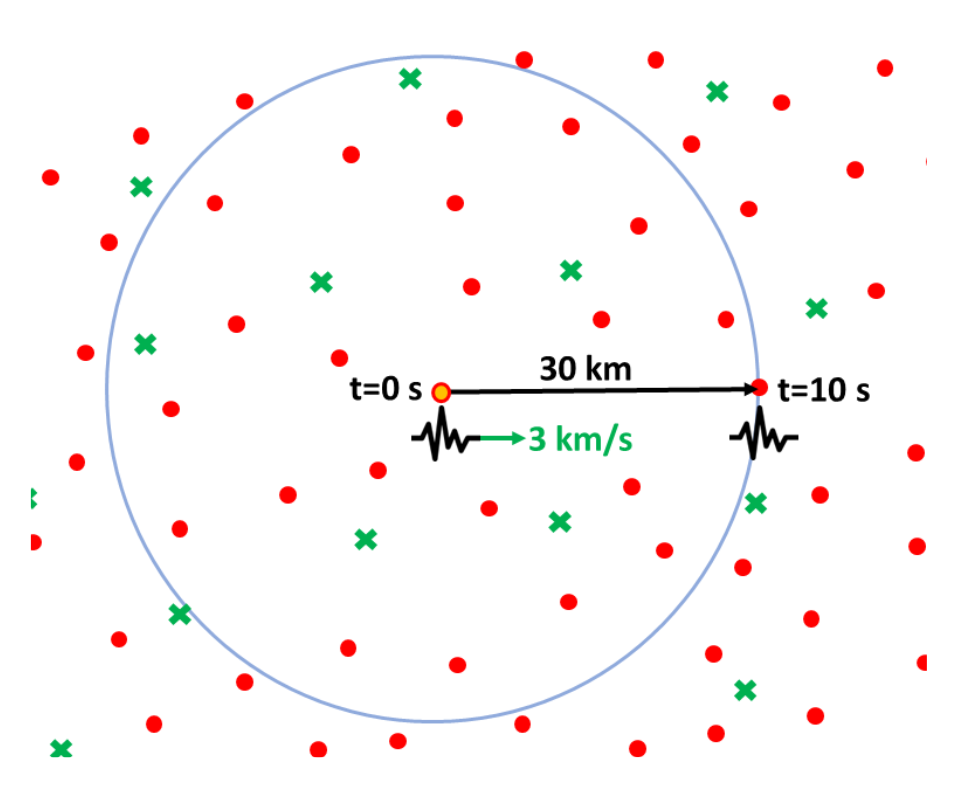
\includegraphics[scale=0.3]{images/30km.png}
    \caption{30km range}
\end{figure}

Our main task is to design an effective communication architecture utilizing LoRa to transmit the earthquake warning message within the specified 30km radius area in approximately 10 seconds. This timeframe accounts for the S-wave's velocity of 3km/s, requiring approximately 10 seconds to cover a 30km distance. Our focus is solely on forwarding the warning packet without the need for any data processing, employing a suitable architecture for this purpose.\\

Let's use the example of secondary waves (S-waves) taking 10 seconds to reach houses 30 kilometers away. If we send our warning message to these houses 7 seconds after the earthquake is sensed by the first node, then the residents of those houses have 3 seconds to take action before the earthquake reaches their location.